%
% Assignment @ DIPT
%
\documentclass[12pt,a4paper]{article}
%
% Set a flag to include or exclude the blue comment boxes.
\usepackage{etoolbox}
\newtoggle{todos}
\toggletrue{todos}
%\togglefalse{todos}
%
% Do only change the row below when changing the template.
% The current date is inserted automatically by command `\date{\today}' below.
\newcommand{\templateVersion}{1.3 -- September 23, 2019}
%
\usepackage[top=2.5cm, bottom=2.5cm, left=2.5cm, right=2.5cm]{geometry} % Sets the size of the document margins
\usepackage[utf8]{inputenc}  % For handling input of special character
\usepackage[T1]{fontenc}  % For better encoding of special characters
%\usepackage[swedish]{babel}  % Uncomment for documents in Swedish
\usepackage{microtype}  % For improved typesetting
\usepackage[hyphens]{url}  % Improved hyphenation of URLs
\usepackage{hyperref}  % For clickable cross-references in the text
\DeclareUrlCommand\email{}  % Formatting of (clickable) email-addresses
\usepackage{enumitem}  % More formatting options for lists
\setlist{topsep=1ex,itemsep=0.5ex,parsep=0pt,partopsep=0pt}  % this sets the vertical spacing between list items and surrounding paragraphs
\usepackage[sort&compress]{natbib}  % Improved formatting of citations
\setlength{\bibsep}{5pt}  % Sets space between two element in the list of references
\usepackage{multirow}  % Required for table cells that span several rows
\usepackage{longtable}  % Necessary for tables that should span several pages
\usepackage{booktabs}  % Addtl. formatting options for tables
%
\usepackage{listings}  % For pretty printing of source code
%
\iftoggle{todos}{%
  % include the blue comment boxes
  \usepackage[color=blue!10,textsize=footnotesize,textwidth=25mm]{todonotes}
}{%
  % exclude the blue comment boxes
  \usepackage[disable]{todonotes}
}  % Contains commands that we pushed to a separate file.

% Please identify COURSE CODE and COURSE NAME.
\newcommand{\theCourse}{PA1234: Course name}

% Please identify ASSIGNMENT NAME.
\newcommand{\theAssignment}{Assignment name, number and/or title}

% *** Do not touch the following lines. BEGIN. ***
\title{\theAssignment\\\vspace{1mm}\footnotesize{Template version \templateVersion}}
\author{\textsc{\theCourse}}
\date{\today}
%
\begin{document}
%
\maketitle
%
\vspace*{-12mm}
% *** END. Do not touch the lines above. ***

% *** BELOW YOU INSERT BASIC INFORMATION ABOUT THE ASSIGNMENT ***
\begin{longtable}{|l|p{12.15cm}|}
\hline
Group name/ID & Group name or ID, in case this is a group exercise \\ 
\hline
Title         & Title of the answer/ solution \\
\hline
Supervisor(s) & Supervisor name(s), if applicable \\
\hline
\end{longtable}


% *** BELOW YOU INSERT DETAILS ABOUT WHO DID WHAT ***
\vspace*{-7mm}
\begin{small}
\begin{longtable}{|l|l|p{10.9cm}|}
\hline
\multirow{4}{*}{Student 1}
 & Name           & Muhammad Saad ur Rehman \\ \cline{2-3}
 & E-Mail         & mure26@student.bth.se \\ \cline{2-3}
 & Program        & DVAMA26h \\ \cline{2-3}
 & Contribution   & Section 4 \\
\hline
\multirow{4}{*}{Student 2}
 & Name           &  Alexander Jamal \\ \cline{2-3}
 & E-Mail         &  aljm19@student.bth.se \\ \cline{2-3}
 & Program        &  DVAMI23h \\ \cline{2-3}
 & Contribution   &  Section 3\\
\hline
\multirow{4}{*}{Student 3}
 & Name           &  Sergii Gavryk \\ \cline{2-3}
 & E-Mail         &  sega24@student.bth.se \\ \cline{2-3}
 & Program        &  PAAMV24h \\ \cline{2-3}
 & Contribution   &  Section 2 and 1.1\\
\hline
\multirow{4}{*}{Student 4}
 & Name           &  Aleksandra Zhurzhenko \\ \cline{2-3}
 & E-Mail         &  alzh24@student.bth.se \\ \cline{2-3}
 & Program        &  PAAMV24h \\ \cline{2-3}
 & Contribution   &  Section 1.2 and 1.3\\
\hline

\end{longtable}
\end{small}

% *** BELOW YOU MAINTAIN THE DOCUMENT HISTORY ***
\begin{small}
\begin{longtable}{|l|p{13.3cm}|}
\hline
\multicolumn{2}{|l|}{\textbf{Submission/change history (latest entry on top)}} \\
\textbf{Date} & \textbf{Changes made} \\
\hline
2019-04-01 & Complemented due to FX. Changes made: ... \\
\hline 
2019-03-22 & Initial submission. \\
\hline 
\end{longtable}
\end{small}

\setcounter{table}{0}  % The tables on the front page shouldn't be counted

% When you need a table of contents, you can uncomment the following line(s)
% \setcounter{tocdepth}{2}  % Sets the level of sections/subsections for the table of contents
% \tableofcontents

\newpage

% *** THE ACTUAL ASSIGNMENT CONTENT STARTS HERE ***
\paragraph{AI Usage} \mbox{} \\
\\
Student 1: Used Claude for writing python scripts.\newline 
\\
Student 2: Used ChatGPT to set up the environment for testing in my local computer, made sure all dependencies were up to date in order to perform the tests more accurately.\newline 
\\
Student 3: I used Claude AI assistance to create scripts for 2.2. I have checked and run scripts in VS Code, where I got test results. I used AI like Chat GPT to learn course material and to critique my work. I have also used google translate with gemini translating function. \newline
\\
Student 4: I used Claude AI to translate some sections in the books and documentation files in Flask repository, to Swedish to understand them more. 

\section{Preparation}
\label{sec:intro}
\subsection{Select and Explore a Software System}
Flask is a lightweight web application framework built on WSGI. It is designed to be both quick and easy to get started with, but it is also designed in a way that allows for the program to scale for more complex applications. Flask started as a simple layer around Werkzeug and Jinja and has since become one of the most popular Python frameworks for web applications. Flask is structured in such a way that it only provides suggestions and never forces any dependencies or any project layout. The developer can choose which tools and libraries to use. (Source: Flask Documentation \cite{flaskdocs} and README) \\ We believe that it is suitable for users such as developers of web applications in Python and developers of add ons. That is, users who want a simple framework where they themselves choose the tools and libraries, as well as functionality outside the core. \\

Link to Flask source code: https://github.com/pallets/flask \\

\noindent \textbf{Key characteristics:}
\begin{itemize}
    \item \textbf{Age:} The project is about 16.5 years old. The first commit was made on April 6, 2010.
    \item \textbf{Repository Size:} \texttt{src/flask} has 24 Python files with 7,563 lines of code (excluding empty lines). The \texttt{tests/} directory has 5,851 lines.
    \item \textbf{Contributors:} 874 different author email addresses have made commits to the repository.
\end{itemize}

\noindent \textbf{Activity over time:}
\begin{itemize}
    \item Most commits were made in 2010 (556), 2014 (465), and 2021 (458).
    \item After 2023, the activity dropped: 172 commits in 2024, 90 in 2025, and 84 in 2026 
\end{itemize}

\subsection{Decide on Relevant Quality Attribute}
\textbf{Quality attribute}\\
Quality attribute that is relevant for our system is Modifiability, Testability and Performance. \\ Modifiability is about changes that happens all the time and that we should be able to lower the cost and risks of it. There are four questions that are necessary to answer for this. The first one is "What can change?" that includes all of the changes related to the system starting from hardware, software ending with its capacity. \cite[8]{SAP} The second one is "What is the likelihood of the change?", describes that it is important to highlight changes that might occur and plan for them. The third one is "When is the change made and who makes it?" it is about the more changes is easy to make, for example trough settings etc, the better because specialist stakeholders are not required. \cite[8]{SAP}. The last one is "What is the cost of the change?" the book divides it in two steps, making a mechanism for changes and using it. Depending on how often you will need changes to be done, you choose if there should be such a thing or not. \cite[8]{SAP} \\
Testability is about how easy it is for the system to show its faults when testing it. That is to say, it shows that system do not hide faults from testers. It also important to be able to recreate faults, so it is possible to show them and find a reason they occurred. \cite[12]{SAP}\\
Performance is about if systems software is capable of time criterion that were established, and how fast it works. Different computer actions requires some time, everything from math calculation and disk connection  to reaching a database or another server. Therefore it is important to think about time when you planning a system. There are different event that should be answered in time, and performance is about how often they occur and how fast do the system answer. \cite[9]{SAP}\\
\textbf{Importance of Modifiability and Testability}\\
 Modifiability is important for the system because it provides a stable web application base with the ability to develop it more, without specific dependencies or project layout. \cite{flaskgit} As it says in 1.1 first commit was made in 2010, from that moment many tools that we use to build web applications may have changed, for example in CHANGES.rst Version 0.10, Released date 2013-06-13 one of the changes were that it now will require Python 2.6 or 2.7 to prepare for Python 3.3 \cite{flaskgit}. It also include over 800 contributors that changed something in the system since it was built, therefore it must include modifiability in order to not destroy any others code.\\
 Testability is important because it have many pull requests that people may do, in order to sort them Flask have some test that must be successful before it goes farther. In flask/docs/contributing there are documentation named  "Contribute to a Pallets Project" that describes how a pull request should be done, is in subsection "Tests" \cite{pullr}. There are information provided on how to run them, for example type "pytests" to test in current environment. To be able to make a successful pull request the test must be as well successful and presented. \\
 \textbf{Performance}\\
 We choose performance because this is a web framework where every request take time. In flask/docs/lifecycle.rst \cite{flaskgit} you can see under "How a Request is Handled" how Flask handle request and generate response, that takes 24 steps where every one takes time.  In \cite{flaskdocs} "Async/await and ASGI support" developer describes that because Flask were built before async were implemented in python it goes with separate coroutines that runs in each threads instead of event loop in main one. It cost more to have threads and makes Flask slower, but is necessary for Flasks code and extensions that were built before async function in python.\cite{flaskdocs} It is a "Compromise" that developers did, and it shows that Performance is import part of the system. 


 \subsection{System Structure and Architecture Decisions}
\label{sec:system_structure}
Decomposition View of Flask


 \textbf{Application base module} - Build web application \\
 \indent sansio\\
 \indent \indent app.py\\
 \indent \indent scaffold.py\\
 \indent \indent blueprints.py\\
 \indent app.py\\
 \indent blueprints.py\\
 \indent config.py\\
 \indent views.py\\

 \textbf{Request module} - responsible to get requests and send response  \\
 \begin{quote}
 wrappers.py\\
 ctx.py\\
 helpers.py
\end{quote} 

 \textbf{Helpers for request module} - tools that helps to send response and remember sessions \\
 \begin{quote}
     globals.py\\
     sessions.py\\
     signals.py\\
     templating.py\\
     json/
 \end{quote}

 \textbf{Helpers for developers module} - tools that makes it easier to use/test application\\
 \begin{quote}
     debughelpers.py\\
     typing.py\\
     logging.py\\
     testing.py\\
     cli.py
 \end{quote}

We divided code in four module because each of it has it own responsibility. First one to build a web application base with objects and configuration, second one is responsible of taking requests and sendning response, third one is to help request module with its work. The last one is to help developers develop their own application. Flask was described as lightweight and easy therefore it provides just base structure with ability to add extensions \cite{flaskgit}. It also fits better with modifiability because each module has its own responsibility and is easier to change without destroying something else.\\
\\ \\ \\ \\ \\ \\ \\ \\ \\ \\ \\ \\ \\ \\ \\ \\ \\ \\ \\ \\ \\

\textbf{Performans view}\\
\begin{figure}
    \centering
    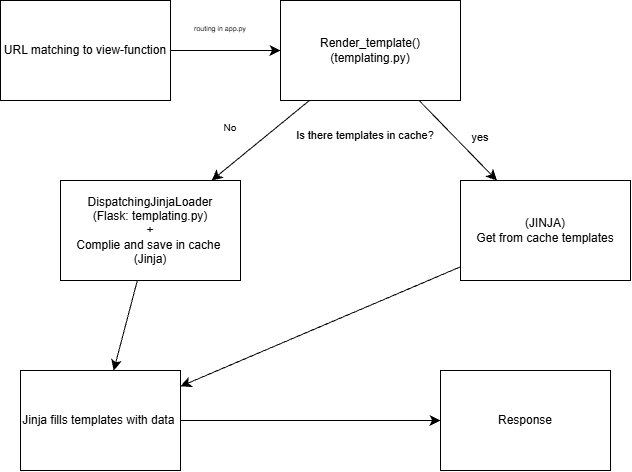
\includegraphics[width=0.5\linewidth]{performanceview.drawio.png}
    \caption{Runtime view of getting template in Flask}
    \label{fig:placeholder}
\end{figure}

This figure describes tactic named "Maintain multiple copies of data" where one of common examples is caching. Meaning with that is to reuse and save data that was recently used\cite[9]{SAP}. This is whats happening here. Jinja that can store cache\url{https://jinja.palletsprojects.com/en/stable/api/#high-level-api} calls from templating.py and after it fills in template that goes back to render\_template(), Flaks makes it to a response\cite{flaskgit} in src/templating.py and src/app.py. Under rubric 4 you can see more about it. 

For decomposition view our decisions where find in flask/src \cite{flaskgit} and README file that describes Flask as lightweight and easy to use. \\
For Runtime view of tactic for Performance, we found have Flask handle request in flask/docs/ lifecycle.rst where 24 steps developers could summarize to 3 which we used in diagram. Also in flask/src we found templating.py with function that calla Jinja, responsible for cache, from function render\_template, and function create\_jinja\_environment from app.py that build Jinja environment for this purpose. 




\section{Modifiability}
We chose modifiability 

• A short definition: What does the metric measure, and how is it obtained?
• A justification: Why does a higher (or lower) value indicate higher quality?
• A limitation: In what situation could the metric be misleading?

\subsection{Metrics}
\subsubsection{Change coupling between modules}
\begin{itemize}
\item \textbf{Definition:}This measures how often files from different modules are changed in the same commit. We look at the four modules from 1.3 and count with git log.
\item \textbf{Justification:} A low value is good, because then you can change one module without having to touch the others.
\item \textbf{Limitation:} The metric can give a wrong picture if a commit changes many files just because the code was reformatted or because dependencies were updated.
\end{itemize}

\subsubsection{Commit size}
\begin{itemize}
\item \textbf{Definition:} This measures how many lines are changed in a regular commit. We take the median and do not count merge commits. This can be obtained with git log --numstat.
\item \textbf{Justification:} Small commits are good, because then changes are made in small steps that can be easier to understand.
\item \textbf{Limitation:} The metric can give a wrong picture if developers merge several commits into one or if the code that was generated and documentation is changed.
\end{itemize}

\subsubsection{Dependencies between modules}
\begin{itemize}
\item \textbf{Definition:} This measures how many times a module imports another, and if there are circular dependencies. We check the import statements with a small script.
\item \textbf{Justification:} Few dependencies and no circles are good, because then the modules are not so tightly connected.
\item \textbf{Limitation:} The metric does not say anything about how strong the dependency is, and imports that only occur when the code is run can be missed.
\end{itemize}

\subsection{Measurements}
For all measurements, we have started from the Flask source code in \texttt{src/flask/} up to commit \texttt{d086db856be187255b8ec61ef409357393020f32} (2026-10-07). The files have been divided into the four modules that we defined in section~\ref{sec:system_structure}.

\subsubsection{Change coupling between modules}
To investigate how often the modules change together, we analyzed the entire Git history for \texttt{src/flask/} via a Python script that ran \texttt{git log}.

Out of a total of 5,562 commits in the project, 401 affected files within our four modules. The results show that:
\begin{itemize}
    \item \textbf{Individual modules:} 299 commits (75\%) affected only a single module.
    \item \textbf{Multiple modules:} 102 commits (25\%) changed code in more than one module at the same time. Of these, 61 commits affected two modules, 24 commits affected three modules, and 17 commits affected all four.
\end{itemize}

The most common pairs of changes were:
\begin{itemize}
    \item \texttt{base} $\leftrightarrow$ \texttt{request}: 58 commits
    \item \texttt{base} $\leftrightarrow$ \texttt{dev\_helpers}: 51 commits
    \item \texttt{base} $\leftrightarrow$ \texttt{req\_helpers}: 39 commits
    \item \texttt{request} $\leftrightarrow$ \texttt{dev\_helpers}: 32 commits
    \item \texttt{request} $\leftrightarrow$ \texttt{req\_helpers}: 31 commits
    \item \texttt{req\_helpers} $\leftrightarrow$ \texttt{dev\_helpers}: 24 commits
\end{itemize}

\subsubsection{Commit size}
The size of the changes was measured by summing added and removed lines per commit for non-merge commits in \texttt{src/flask/} (via \texttt{git log --no-merges} and \texttt{git show --numstat}).

The measurement was based on the 411 commits that actually contained code changes in the modules:
\begin{itemize}
    \item \textbf{Median:} 10 lines per commit
    \item \textbf{Mean:} 75.6 lines
    \item \textbf{Quartiles:} P25 = 3 lines, P75 = 41 lines
    \item \textbf{Largest change:} 8,161 lines in a single commit
\end{itemize}
The average is significantly skewed by a few very large changes, making the median of 10 lines a more accurate measure of a typical commit size.

The number of import statements between the modules was distributed as follows:
\begin{itemize}
    \item \texttt{base} $\rightarrow$ \texttt{req\_helpers}: 40 imports
    \item \texttt{base} $\rightarrow$ \texttt{request}: 30 imports
    \item \texttt{base} $\rightarrow$ \texttt{dev\_helpers}: 12 imports
    \item \texttt{request} $\rightarrow$ \texttt{req\_helpers}: 11 imports
    \item \texttt{req\_helpers} $\rightarrow$ \texttt{request}: 8 imports
    \item \textbf{Other directions:} between 1 and 6 imports each
\end{itemize}

\subsection{Discussion}
Our measurements show that Flask can be both good and less good when it comes to modifiability. The positives are that changes are often small, this is shown by the median being only 10 lines per commit, which makes it easier to understand and test changes. In addition, the measurements showed that 75\% of all commits affect only a single module. This means that there is a module division, so you can work in one module without having to touch the others.

At the same time, these modules are hard-coupled with each other. So that all modules import from all others so there are dependencies. The base module is often changed together with request and dev\_helpers. This means that changes to the core can affect other parts of the code, and increases the risk of errors.

In summary, small commits and the high proportion of module changes make it easier to make changes locally. However, since there are many dependencies between modules, you should be careful when changing the core, so as not to break anything else. A possible improvement could be to reduce the dependencies from the base module or to make the boundaries between modules clearer.


\section{Testability}
\label{sec:testability}
We chose testability to evaluate how easily and effectively Flask tests applications.
\subsection{Metrics}
\begin{itemize}
\item\textbf{Code Health (1-10):} To have an overview of the quality of the code, lower code health can indicate code that is hard to maintain and test.
\item\textbf{Code coverage (\%):} Coverage shows how much of the application code is executed and can indicate whether the tests run the full code or misses parts of it.
\item\textbf{Test success rate (\%):} To check whether the test files are being executed as intended using Pytest.
\end{itemize}

\subsection{Measurements}
First we forked the repository of Flask and ran the environment on our local computer, using the analysis function that CodeScene provides, we were able get the Code Health value of the repository as a whole. Since we are looking into testability we found that the code health for the test suite within the repository was 8.7/10. In figure 2 can be shown the code health for the different test files where most of them are healthy (10/10 code health) with the exception of "test\_basic.py" which is connected to the application and other test files, and "test\_blueprints.py".\newline
To measure the code coverage of flasks we used the coverage function within pytest-cov and ran the coverage test on the Flask application that resulted in a total coverage of 95\%.
Finally, in order to try the test success rate we used the pytest command to let the tests run. After setting up the environment to get all functions work properly, the result was that the 491 tests ran successfully and passed while 3 were skipped, with the total amount it took being 2.50 seconds. The success rate of the tests that have been run is 100\%.
\begin{figure}
    \centering
    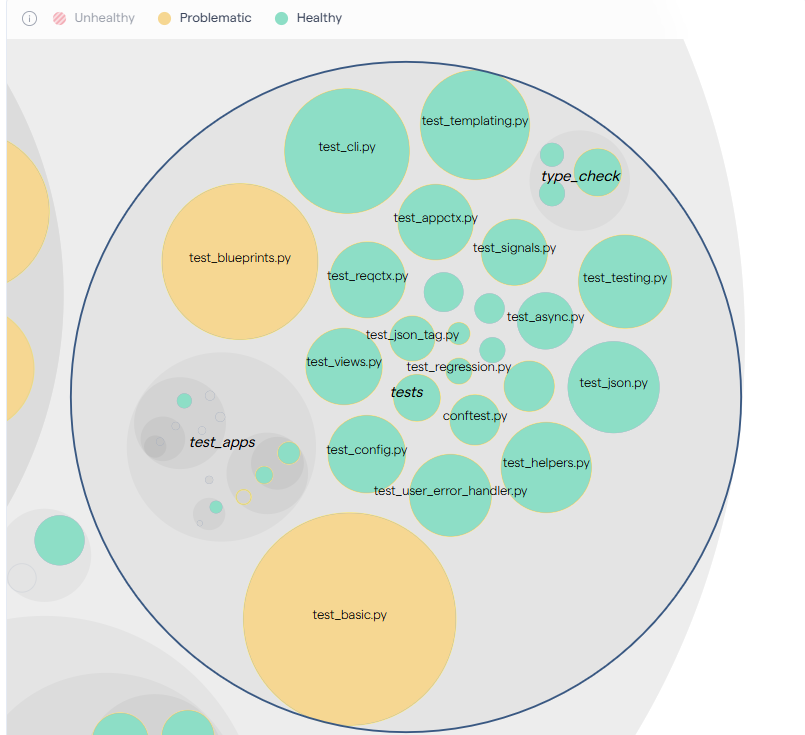
\includegraphics[width=0.5\linewidth]{code_health_tests.png}
    \caption{Code Health for the test suite}
    \label{fig:code_health}
\end{figure}
\subsection{Discussion}
The results suggest that the Flask project has a well maintained and exercised test suite. The CodeScene code health of the test files, with a result of 8.7/10, indicate a fairly strong code health within the test files. The test files with a score of 10/10 in code health can be overlooked but further investigation with the test files "test\_basic.py" and "test\_blueprints.py" is needed to improve their code health. \newline
The code coverage of 95\% indicate that when the application is being tested, the grand majority of lines are being run, which is a positive thing for the codes testability, showing that the tests cover the vast majority of the application.\newline
The test success rate showing 491 tests executing and passing, with 3 being skipped and no failures indicates a high success rate, meaning that the tests running in the right environment with the dependencies needed can successfully pass and run.\newline
Taken into account the three measurements, we can see that Flask repository has a fairly positive testability, with only a few test files needed to be looked over to strengthen the overall testability of the system. Alas testability is much broader than this and some important aspects may have been overlooked such as testing the units individually. 




\section{Performance}
\label{sec:performance}
We chose performance to see how quickly a Flask app handles requests and how much memory it uses. Our test compares the same page with template caching on and off.

\subsection{Metrics}
\label{sec:performance-metrics}
\begin{itemize}
\item \textbf{P95 response time (ms):} About 95\% of requests finish within this time, as reported by Locust. A lower value means less waiting. It leaves out the slowest 5\% of requests, and the result can be affected if Locust is too busy.
\item \textbf{Throughput (requests/s):} Locust reports how many requests finish each second. A higher number means the app handles more work, as long as the responses are correct. Locust itself may limit the rate, so we check its CPU warnings and failed requests too.
\item \textbf{Peak sampled memory (MiB):} We take the highest app-container reading from \texttt{docker stats}. Using less memory leaves more available for other work. The reading includes Gunicorn, Python, and the cache. Short peaks between readings can be missed. Docker’s Linux reading excludes some file-cache memory.\footnote{\url{https://docs.docker.com/reference/cli/docker/container/stats/}}
\end{itemize}

\subsection{Measurements}
\label{sec:performance-measurements}
We used Flask 3.1.3, Jinja2 3.1.6, Python 3.13.16, Gunicorn 26.2.0 and Locust 2.46.7. The app and Locust ran in separate Docker containers on an ARM64 Mac connected to AC power. Docker had four CPUs and about 5.8 GiB of memory. The app was limited to one CPU and 1 GiB of memory, with no swap, using one Gunicorn worker and one thread.

Our app has one page with a list of 20 numbers. We set the Jinja cache size to 400 for caching on and 0 for caching off, and disabled automatic template reload in both cases.

Flask uses Jinja to render our page. With caching on, Jinja keeps the compiled template in memory and reuses it for later requests. This avoids loading and compiling the same template again. We compare caching on and off to measure the effect of this reuse. The page is still built for every request in both cases.\footnote{\url{https://jinja.palletsprojects.com/en/stable/api/}}

We started a fresh app container for each run. After a 15-second warm-up, we measured for 60 seconds. Two Locust workers shared ten simulated users, who sent requests without pauses. Locust reset the statistics once the users had started. We checked each response for status 200 and 20 list items. We ran each cache setting three times, in the order shown in the table.

P95 and throughput come from the aggregate row in \path{locust_stats.csv}. Peak memory comes from \path{memory.log}, which also covers the measurement client’s startup and shutdown. The summary script calculates each metric’s median, the middle value of its three runs.

\begin{table}[htbp]
\centering
\caption{Results in run order. Memory is the highest sampled value per run.}
\label{tab:performance-results}
\small
\begin{tabular}{llrrr}
\toprule
Run & Cache & P95 (ms) & Requests/s & Memory (MiB) \\
\midrule
1 & on & 7 & 2173.0 & 64.09 \\
2 & off & 11 & 1223.9 & 42.71 \\
3 & off & 11 & 1254.3 & 44.33 \\
4 & on & 5 & 2513.2 & 42.71 \\
5 & on & 10 & 1788.3 & 43.90 \\
6 & off & 12 & 1267.7 & 42.80 \\
\midrule
Median & on & 7 & 2173.0 & 43.90 \\
Median & off & 11 & 1254.3 & 42.80 \\
\bottomrule
\end{tabular}
\end{table}

All 613,107 measured requests passed the response checks. The app did not restart or run out of memory. Our earlier tests had CPU warnings from Locust, so we repeated all six runs with two workers. These new runs had no CPU warnings and are the ones shown in the table.

The scripts, settings and results are included with this assignment in the \path{qa3/} folder. Scripts are in \path{qa3/scripts/}, settings are in \path{qa3/compose.yaml}, and results are in the six folders listed in \path{qa3/data/environment.txt}. Each run includes logs, package versions, settings and the measured code version in \path{commit.txt}.

To repeat the test, open the main assignment folder containing the \path{justfile}. Run \texttt{just build} once, then \texttt{just start on} or \texttt{just start off}, followed by \texttt{just bench} for each run. Use \texttt{just stop} when finished. The command \texttt{just summary} reads the listed run folders; update the list to summarise a new batch.

\subsection{Discussion}
\label{sec:performance-discussion}
We compared caching on and off in three run pairs: runs 1--2, 3--4 and 5--6. In every pair, caching gave a lower P95 response time and higher throughput. The median P95 was 7 ms with caching and 11 ms without it. The median throughput was 2173.0 requests/s with caching and 1254.3 requests/s without it. These results support keeping the compiled template in memory so Jinja can reuse it.

The memory results were less clear. Peak sampled memory was higher with caching in two pairs and lower in one. The median was 43.90 MiB with caching and 42.80 MiB without it. The first cached run reached 64.09 MiB, but we do not know why. We measured the whole app container, so we cannot tell how much memory the cache itself used.

The results also varied between runs. With caching, throughput ranged from 1788.3 to 2513.2 requests/s. We tested only one small template with ten simulated users on a shared laptop. Other apps or test conditions may give different results. These tests do not show Flask's maximum capacity. We also had no performance target, so we can compare the two settings but cannot say whether the app meets a required response time or throughput.

For this app, we would keep Jinja's template cache enabled because it improved response time and throughput in all three comparisons. Our results give us no reason to replace the caching design. A next test could use more templates and different user counts. Running Locust on a separate machine would reduce competition between the app and Locust for the laptop's CPU and memory.

%\section{More information}
%\label{sec:more}
%For more details on report writing, please refer to \textit{Rapportskrivning för ingenjörer} \cite{nilsson2018rapport} (Swedish only), which can be downloaded from the library's Writing Guide (Skrivguiden)\footnote{\url{http://skrivguiden.se/resurser/bth-resurser/} (Swedish) or \url{http://writingguide.se/resources/bth-resources/} (English)}.  There are also of resources for learning \LaTeX\ on \url{https://www.overleaf.com/learn}. There are also numerous free guides for learning \LaTeX\ on the Internet, e.g., \cite{oetiker2011not}.

% All references are stored in a separate bib-file: ass-refs.bib
%\clearpage
\small
\bibliographystyle{plain}
\bibliography{ass-refs}

\end{document}
